\newpage
\chapter{Cluster-Matching-Based Method For Video Face Recognition}
\label{chap:face_recognition}

In this chapter, we describe the first application we investigated using the \emph{Video Face Clustering} method.
%%
We propose a cluster-matching-based approach for video face recognition where \emph{face clustering} is used to group faces in both the face dataset and in the target video~(video face clustering).
%%
Consequently, classes do not have to be previously known, and the effort spent with annotations is significantly reduced --- as it is done over clusters instead of single images.
%%
Face recognition becomes a task of comparing clusters from the dataset with the ones extracted from images or video sources.
%%
Therefore, our approach is easily scalable.

This chapter is structured as follows. In Section \ref{sec:recognition_method}, we detail our proposed method, followed by two sections with experiments: 
%%
Section \ref{sec:recognition_clustering_validation}, regarding the clustering methods we use, and 
%%
Section \ref{sec:recognition_matching_validation}, with the experiments with our matching heuristic.
%%
Section \ref{sec:recognition_video_evaluation} is devoted to the overall evaluation of our method and, finally, 
%%
in Section \ref{sec:recognition_discussion}, we conclude this chapter by discussing our results.

\section{Proposed Method}
\label{sec:recognition_method}


Figure \ref{fig:cluster_matching} shows our proposed approach.

\begin{figure*}[!ht]
    \centering
    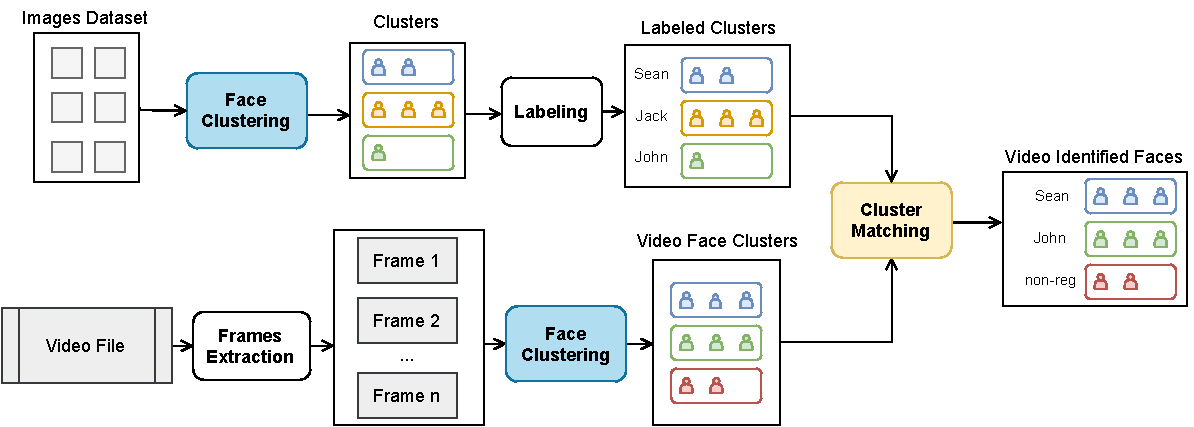
\includegraphics[width=\textwidth]{img/face_clustering/cluster_matching_process.pdf}
    \caption{Cluster-Matching based Method for Video Face Recognition.}
    \label{fig:cluster_matching}
\end{figure*}

In our approach we use \emph{face clustering} in an images dataset and in the referenced video. Then, the clusters of the images dataset are labeled. 
%%
In the \textit{Labeling} step, we assign labels~(identities) to represent the clusters.
%%
A label can be anything that represents the faces present in the cluster, e.g. a name or an id number. 
%%
Using this pipeline, instead of having to label every single face for constructing a labeled dataset, it is only necessary to label each generated cluster.
%%
Consequently, all the faces present in a cluster are assigned to the same label. 
%%
Hence, the complexity of labeling becomes a function dependent on the number of clusters, which is at most as great as the number of individuals.
%%
At the end of this step, we have a dataset of \emph{Labeled Clusters}.


Next, we perform \emph{Cluster Matching} where the clusters from the image dataset and from the video are matched using a heuristic based on clusters distance.

The \textit{Cluster Matching} step receives the set of clusters from the video and the set of labeled clusters, which is used as a reference for recognizing the clusters (and consequently the faces) in the video.
%%
%%
We designed a method based on cluster distance for performing this recognition.
%%
We compare each candidate cluster in the video with each of the labeled clusters in the reference dataset, using what we call a \emph{cluster embedding}. This \emph{cluster embedding} is computed for both the candidate cluster in the video and the reference cluster in the labeled dataset.
%%
The \emph{cluster embedding} maps each cluster to a vector in the embedding space of the face embeddings.
%%
In the experiments, we evaluate two ways of obtaining a \emph{cluster embedding}.

Let $q$ denote the \emph{cluster embedding} of the query cluster, where $q~\in~\mathbb{R}^{n}$, in which $n$ is the dimension of the embedding space.
%
Let $K$ denote the set of labeled clusters. For each $k~\in~K$, let $c_k$ denote the \emph{cluster embedding} of $k$. 
%
We compute a similarity function of $q$ and each $c_k$ for $k~\in~K$. 
%%
This similarity function is based on the Root Mean Square Error~(RMSE) function, which is largely used for computing embeddings distances in machine learning techniques.\footnote{https://www.sciencedirect.com/topics/engineering/root-mean-square-error}
%%
We decided to use the inverse of the RMSE since we want to return larger values for clusters that are closer to $q$, to be able to use these values to compute a probabilistic distribution:

\begin{equation}
\label{equation:similarity_raw}
    s_{q,k} = \frac{1}{\sqrt{\frac{1}{n}\sum_{i=0}^{n}{(q_i-c_{k,i})^2}}}
\end{equation}

Since we are not interested in clusters that too distant from $q$, we define $\overline{s}_{q,k}$ that considers only the $\alpha$ largest $s_q$ values. The $\alpha$ value is a parameter that we further evaluate in this work. 
Thus, our similarity function becomes

\begin{equation}
\label{equation:similarity}
    \overline{s}_{q,k} = \begin{cases}s_{q,k} & \text{if}~s_{q,k}~\in max_{\alpha(s_q)}\\0 & \text{otherwise}\end{cases}
\end{equation}

Given the similarity~$\overline{s}_{q,k}$, we compute the probability of $q$ being a match with each labeled cluster using the \emph{softmax} function.
%%
This function takes as input a vector of real numbers and normalizes it into a probability distribution consisting of probabilities proportional to the exponential of the input numbers. 
It is defined as

\begin{equation}
\label{equation:probability}
    p_{q,k} = \frac{e^{\overline{s}_{q,k}}}{\sum_{j~\in~K}{e^{\overline{s}_{q,j}}}}
\end{equation}

Finally, we define the function $\sigma$ that, given a \emph{cluster embedding} query $q$, returns the cluster in the labeled clusters whose \emph{cluster embedding} is more likely to have a match with the query if it has a probability greater than $0.5$. Otherwise, the query is assigned as being a match with none of the clusters ($\text{\o}$ is given as result). The $\sigma$ function is defined as follows.

\begin{equation}
\label{equation:sigma}
    \sigma{(q)} = \begin{cases}argmax(p_q) & if~~~p_{q,argmax(p_q)}~>~0.5\\\text{\o} & otherwise\end{cases}
\end{equation}

The $argmax$ function applied over $p_q$ returns the cluster $k$ whose probability of $q$ being a match with it is the greatest. 
%%
We observed that when a cluster has faces that belong to a person present in the labeled clusters, the probability tends to be higher for one single labeled cluster.
%%
However, when the person is not in any of the labeled clusters, the probability tends to be more distributed among different labeled clusters.
%%
For that reason, when none of the labeled clusters has a probability greater than $0.5$, we say that the query cluster does not match any of the labeled clusters.
%%
Hence, the person in the video represented by the query cluster is not present in the labeled clusters.

\section{Faces Clustering Validation}
\label{sec:recognition_clustering_validation}

\section{Cluster-Matching Validation}
\label{sec:recognition_matching_validation}

\section{Video Face Recognition Evaluation}
\label{sec:recognition_video_evaluation}

\section{Discussion}
\label{sec:recognition_discussion}
